\documentclass{beamer}

\usepackage{adjustbox}
\usepackage{tikz}
\usetikzlibrary{calc}

\newcommand{\beff}{\ensuremath{b_{\mathrm{eff}}}}
\newcommand{\bhom}{\ensuremath{b_{\mathrm{hom}}}}
\newcommand{\bmin}{\ensuremath{b_{\mathrm{min}}}}

\title{Effective slip lengths for Stokes flow \\ over rough, mixed-slip surfaces}
\subtitle{PhD Defense Presentation}

\author{Nat Lund \\ 300055048}
\institute{Victoria University of Wellington}
\date{Friday 12th September 2014}

\begin{document}

\begin{frame}
\maketitle
\end{frame}


\begin{frame}
\begin{itemize}
\item Elevator speech
\item Regimes of Applicability, and What Next?
\item Limitations of Homogenization
\end{itemize}

\end{frame}

\begin{frame}{Motivation}
Lab-on-a-chip

\begin{center}
\includegraphics[scale=0.5]{lab-on-chip.jpg}
\end{center}

Very small pipe: friction dominates

\vspace{1em}
How to reduce friction?
\end{frame}

\begin{frame}{Slippery Surfaces}

\begin{center}
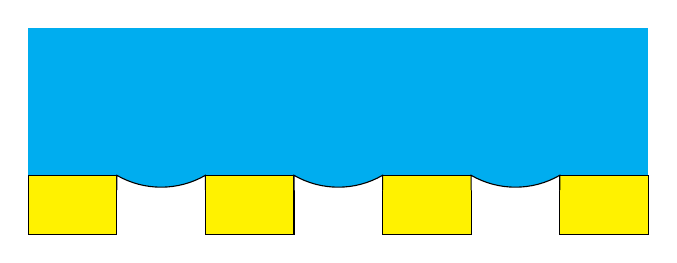
\begin{tikzpicture}[scale=0.75]

\coordinate (slotwidth) at +(1.5,0);
\coordinate (topright) at ($7*(slotwidth) + (0,2.5)$);
\fill[cyan] (0,-0.23) rectangle (topright);

\path (slotwidth) ++(0,-1) coordinate (box);

\foreach \n in {0,1,2,3}
    \draw[fill=yellow] ($2*\n*(slotwidth)$) rectangle +(box);

\foreach \n in {1,3,5}
\draw[fill=white] ($\n*(slotwidth) + (0,-0.25) $) -- ++(0,0.25) arc (240:300:1.5) -- +(0,-0.25);

%\renewcommand{\baselinestretch}{1.0}

%\path ($2*(slotwidth) $) -- node[align=center] {No\\ Slip} +(box);
%\path ($3*(slotwidth) + (0,-0.2)$) -- node[align=center] {Perfect\\ Slip} +(box);

%\path (0,0) -- node[align=center] {Flow Parallel to Slots\\ (Into Page)} (topright);

%\foreach \n in {1,3,5}
%    \draw[fill=cyan] ($\n*(slotwidth)$) arc (240:300:1.5);
    
\end{tikzpicture}
\end{center}

\begin{itemize}
\item Holes on the wall of the pipe
\item Air bubbles trapped in holes
\item Water slips over top of air bubble
\item Friction reduced:  How much?
\end{itemize}

\end{frame}


\begin{frame}{Slip Length}

\begin{center}

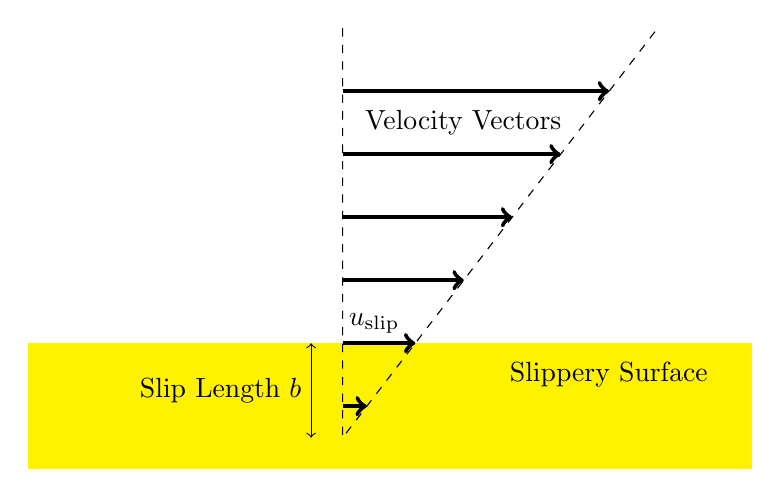
\begin{tikzpicture} [scale=0.8]   [> = stealth]

%\filldraw[fill=yellow, draw=black] (-1.5,5) rectangle ++(11.5,1);
\fill[color=yellow] (-1.5,0) rectangle ++(11.5,-2);

%\node at (-1,5.5) [right] {Top Plate, Velocity $u_{P}$};
\node at (3.7,3.5) [right] {Velocity Vectors};
\node at (6,-0.5) [right] {Slippery Surface};

%\draw [->, ultra thick] (3.5,5.5) -- +(5,0);

%\draw [<->] (1,0) -- node[right] {$P$} +(0,5); 

% x,z axes
%\draw [<->] (1,3) -- node[left] {$z$} ++(0,-2) -- node[below] {$x$} +(2,0); 

\foreach \z in {-1,0,1,2,3,4}
  \draw [->, ultra thick] (3.5,\z) -- +(\z*0.76923 + 1.1545 ,0);

\draw [dashed] (3.5,5) -- +(0,-6.5) -- +(5,0); 

\draw [<->] (3,0) -- node[left] {Slip Length $b$} +(0,-1.5); 

\node at (4,0)[above] {$u_{\mathrm{slip}}$};

\end{tikzpicture}

\end{center}

Single parameter to express the friction of a surface.

\end{frame}


\begin{frame}{Effective Slip Length}

\begin{center}

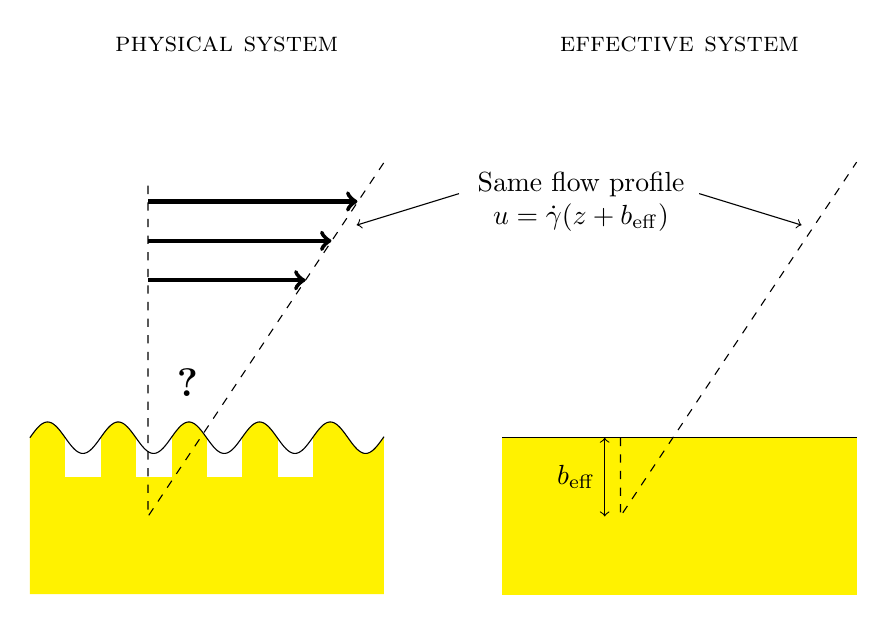
\begin{tikzpicture}

\coordinate (ori) at (0,0);
%\fill[color=cyan] (ori) ++(0,-1) rectangle ++(4.5,5);
\fill [color=yellow,domain=0:4.5,samples=200] plot (\x,{ 0.2 * sin(7*\x r)} ) -- ++(0,-2) -| (ori);
\fill [color=white] (ori) ++(0.45,0) rectangle ++(0.45,-0.5);
\fill [color=white] (ori) ++(1.35,0) rectangle ++(0.45,-0.5);
\fill [color=white] (ori) ++(2.25,0) rectangle ++(0.45,-0.5);
\fill [color=white] (ori) ++(3.15,0) rectangle ++(0.45,-0.5);
\draw [domain=0:4.5,samples=200] plot (\x,{ 0.2 * sin(7*\x r)} );

\draw[dashed] (ori) ++(1.5,3.2) -- ++(0,-4.2) -- ++(3,4.5);
\draw[->, ultra thick] (ori) ++(1.5,2) -- ++(2,0);
\draw[->, ultra thick] (ori) ++(1.5,2.5) -- ++(2.33,0);
\draw[->, ultra thick] (ori) ++(1.5,3) -- ++(2.66,0);
\node at (2,0.7) {\Large{\textbf{?}}};
%\node at (2.5,4) {Smooth Couette flow in far field};


\coordinate (ori) at (6,0);
%\fill[color=cyan] (ori) ++(0,-1) rectangle ++(4.5,5);
\fill[color=yellow] (ori) rectangle ++(4.5,-2);
\draw (ori) -- ++(4.5,0);

\draw[dashed] (ori) ++(1.5,0) -- ++(0,-1) -- ++(3,4.5);
\draw[<->] (ori) ++(1.3,0) -- node[left] {\beff} ++(0,-1);

\draw[<-] (4.15,2.7) -- ++(1.3,0.4);
\draw[<-] (9.8,2.7) -- ++(-1.3,0.4);
\node at (7,3) [align=center] {Same flow profile\\$u = \dot{\gamma} (z + \beff)$};

\node at (2.5,5) {\textsc{physical system}};
\node at (8.25,5) {\textsc{effective system}};


\end{tikzpicture}

\end{center}

\end{frame}


\begin{frame}{Mathematical Model}

\begin{center}

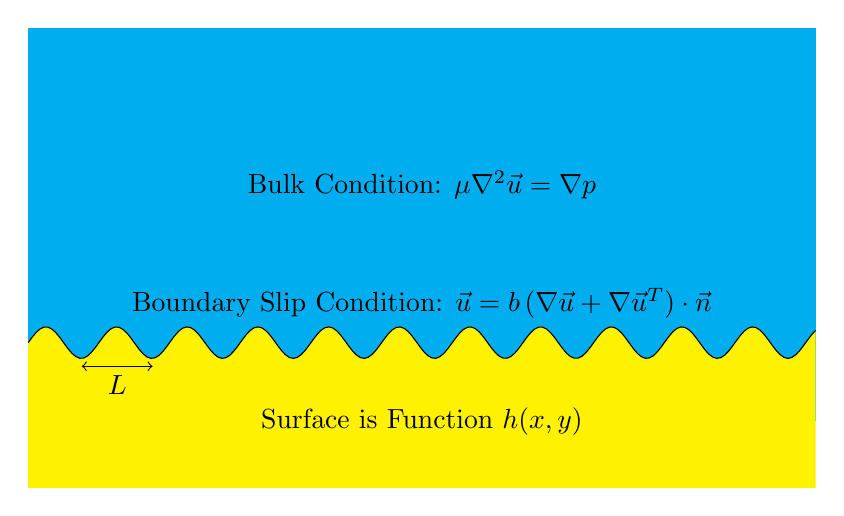
\begin{tikzpicture}
\fill[color=cyan] (0,-1) rectangle (10,4);

\node at (5,2) {Bulk Condition: $\mu \nabla^2 \vec{u} = \nabla p$};
\node at (5,0.5){Boundary Slip Condition:  $\vec{u} = b \, (\nabla \vec{u} + \nabla \vec{u}^T) \cdot \vec{n}$};

\fill [color=yellow,domain=0:10,samples=200] plot (\x,{ 0.2 * sin(7*\x r)} ) -- ++(0,-2) -| (0,0);
\draw [domain=0:10,samples=200] plot (\x,{ 0.2 * sin(7*\x r)} );

\node at (5,-1) {Surface is Function $h(x,y)$};

\draw[<->] (0.68,-0.3) --node[below] {$L$} ++(0.9,0);

\end{tikzpicture}

\end{center}

\end{frame}

\begin{frame}{Solving}

\textbf{Homogenization:}

Thought experiment about what happens when the period $L$ becomes infinitely small.

\begin{center}

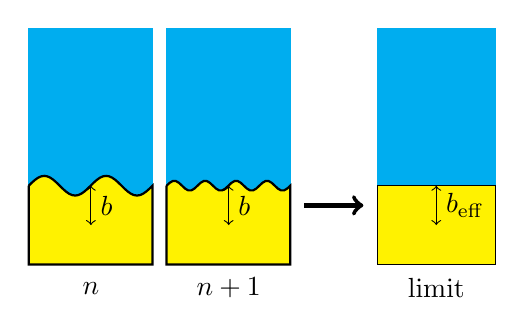
\begin{tikzpicture}[scale=0.5]
%\draw [thick, domain=0:6.283,samples=41] plot (\x, { sin(\x  r) });

\draw [fill=cyan,color=cyan] (0,-1) rectangle ++(3.1416, 5);
\draw [fill=cyan,color=cyan] (3.5,-1) rectangle ++(3.14, 5);
\draw [fill=cyan,color=cyan] (8.85,-1) rectangle ++(3, 5);



\draw [fill=yellow, thick, domain=0:3.1416,samples=41] plot (\x, { sin(4*\x  r)/4 })
 |- (0,-2) -- (0,0);

\draw [fill=yellow, thick, domain=0:3.1416,samples=41] plot (\x+3.5, { sin(8*\x  r)/8 })
 |- (3.5,-2) -- (3.5,0);

\draw[->, ultra thick] (7,-0.5) -- ++(1.5,0);

\draw[fill=yellow] (8.85,0) rectangle ++(3,-2);

\draw[<->](1.578,0) -- node[right]{$b$} ++(0,-1);
\draw[<->](5.078,0) -- node[right]{$b$} ++(0,-1);
\draw[<->](10.35,0) -- node[right]{$\beff$} ++(0,-1);

\node at (1.578,-2.6) {$n$};
\node at (5.078,-2.6) {$n+1$};
\node at (10.35,-2.6) {limit};

%\draw[<->] (7,0) -- node[right]{$P$} ++(0,4);

\end{tikzpicture}

\end{center}

\textbf{Perturbation:}

Think of system as `perturbed' slightly away from a well-known system (with known solution).

\end{frame}

\begin{frame}{Homogenized Solution}

\begin{equation}
\beff = \left< \frac{\sqrt{1 + \lvert \nabla h \rvert^2}}{b} \right> ^{-1}
\label{eq:homogharm}
\end{equation}

Harmonic mean of intrinsic slip lengths, weighted by area of contact:

\begin{center}
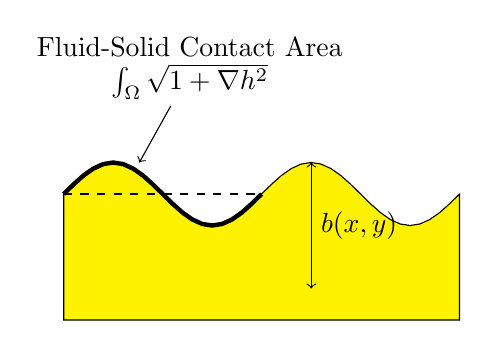
\begin{tikzpicture}[scale=0.8]

%samples = 4n per period + 1
\draw [fill=yellow, domain=0:6.283,samples=41] plot (\x, {sin(2*\x  r)/2 })
 |- ++(0,-2) -| (0,0); 
\draw [ultra thick, domain=0:3.1416,samples=21] plot (\x, {sin(2*\x  r)/2 });

\draw[dashed] (0,0) -- ++(3.1416,0);

\node at (2,2) [align=center]{Fluid-Solid Contact Area\\ $\int_{\Omega} \sqrt{1 + \lvert \nabla h \rvert^2} $};
\draw [<-] (1.2,0.5) -- ++(0.5,0.9);

\draw[<->] (3.93,0.5) -- node[right] {$b(x,y)$} ++(0,-2);

\end{tikzpicture}
\end{center}

\end{frame}

\begin{frame}{Perturbative Solutions}

Replicates homogenized solution for special case of flat surface:
\begin{equation}
\beff = \left< \frac{1}{b} \right>^{-1}
\end{equation}

\vspace{1em}
Where $b$ is much smaller than other length scales, $\beff$ is simple average:
\begin{equation}
\beff = \left< b \right>
\end{equation}

\end{frame}

\begin{frame}{Regimes of Applicability}

Harmonic mean $\beff$ is excellent approximation when period $L$ is much smaller than other lengths, slip lengths $b$ and domain size $P$.
\begin{equation}
\beff = \left< \frac{1}{b} \right>^{-1}
\quad \text{when} \quad
L \ll b, P
\end{equation}

(Still good approximation even if $L \sim b \ll P$.)

\vspace{1em}
Simple mean good approximation when slip lengths $b$ much smaller than other lengths:
\begin{equation}
\beff = \left< b \right>
\quad \text{when} \quad
b \ll L, P
\end{equation}

\end{frame}


\begin{frame}{Regimes and Results}
\begin{adjustbox}{scale=0.55, center}

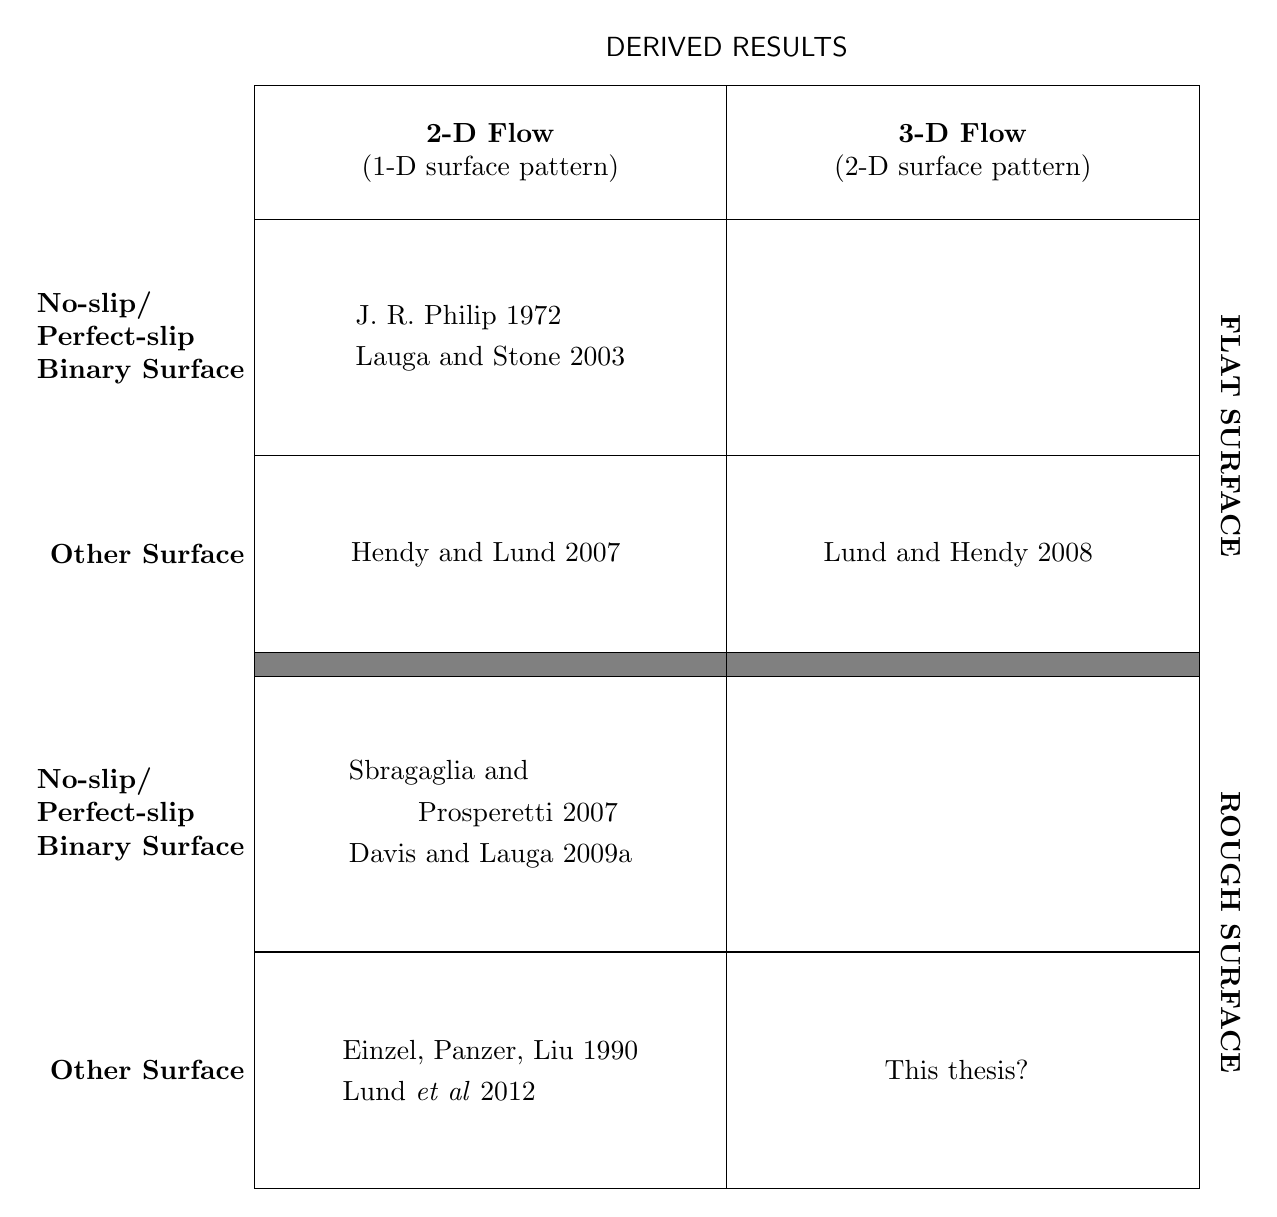
\begin{tikzpicture}

% Manually define half width of table.
\path (6,0) coordinate (midway);

% Manually define row heights.
\path (0,3) coordinate (flatbinary);
\path (0,2.5) coordinate (flatother);
\path (0,3.5) coordinate (roughbinary);
\path (0,3) coordinate (roughother);

\path (0,0.3) coordinate (sepwidth);

\path (0,1.7) coordinate (labelbox);

%%%%%%%%%%%%%%%%%%%%%%%%%%%%%%%%%%%%%%%%% Tikz calculates all other points...
% Bottom left corner is origin (0,0)
\path (0,0) ++(midway) coordinate (midbottom);

\path (0,0) ++(roughother) coordinate (lowdiv);
\path (lowdiv) ++(roughbinary) coordinate (belowsep);
\path (belowsep) ++(sepwidth) coordinate (abovesep);
\path (abovesep) ++(flatother) coordinate (highdiv);
\path (highdiv) ++(flatbinary) coordinate (celltop);
\path (celltop) ++ (labelbox) ++(midway) coordinate (topmid);
\path (topmid) ++(midway) coordinate (topright);


%%%%%%%%%%%%%%%%%%%%%%%%%%%%%%%%%%%%%%% Draw all boxes and lines...
\draw (0,0) rectangle (topright);
\draw (celltop) -- ++(midway) -- ++(midway);
\draw (highdiv) -- ++(midway) -- ++(midway);
\draw [fill=gray] (abovesep) ++(midway) ++(midway) rectangle (belowsep);
\draw (lowdiv) -- ++(midway) -- ++(midway);
\draw (topmid) -- (midbottom);

%%%%%%%%%%%%%%%%%%%%%%%%%%%%%%%%%%%%%%% Add flow type labels.
\path (celltop) --         coordinate[midway] (2Dlabel) (topmid);
\path (2Dlabel) ++(midway) coordinate (3Dlabel);
\node at (2Dlabel)[align=center] {\textbf{2-D Flow}\\(1-D surface pattern)};
\node at (3Dlabel)[align=center] {\textbf{3-D Flow}\\(2-D surface pattern)};

%%%%%%%%%%%%%%%%%%%%%%%%%%%%%%%%%%%%%%   Labels for surface types
\path (abovesep) -- coordinate[midway] (midflat) (celltop);
\path (0,0) --      coordinate[midway] (midrough) (belowsep);
\path (midflat) ++(midway) ++(midway) ++(0.4,0) coordinate (flatlabel);
\path (midrough) ++(midway) ++(midway) ++(0.4,0) coordinate (roughlabel);
\node at (flatlabel)  [rotate=270] {\textbf{FLAT SURFACE}};
\node at (roughlabel) [rotate=270] {\textbf{ROUGH SURFACE}};

%%%%%%%%%%%%%%%%%%%%%%%%%%%%%%%%%%%%%%%%%%%%%%%%%%%  Points in middle of rows...
\path (celltop)  -- coordinate[midway] (row1) (highdiv);
\path (highdiv)  -- coordinate[midway] (row2) (abovesep);
\path (belowsep) -- coordinate[midway] (row3) (lowdiv);
\path (lowdiv)   -- coordinate[midway] (row4) (0,0);

%%%%%%%%%%%%%%%%%%%%%%%%%%%%%%%%%%%%%%%%%%%%%%  Labels for Binary or Other surface types.

\renewcommand{\baselinestretch}{1.0}

\node at (row1) [left, align=left] {\textbf{No-slip/} \\ \textbf{Perfect-slip}\\
										\textbf{Binary Surface}};
\node at (row2) [left, align=left] {\textbf{Other Surface}};
\node at (row3) [left, align=left] {\textbf{No-slip/} \\ \textbf{Perfect-slip}\\
										\textbf{Binary Surface}};
\node at (row4) [left, align=left] {\textbf{Other Surface}};

\renewcommand{\baselinestretch}{1.24}

%%%%%%%%%%%%%%%%%%%%%%%%%%%%%%%%%%%%%%%%%%%%%%%%%  Locations of Text nodes...
%%%%%%%%%%%%  2-D Flow
\path (row1) -- coordinate[midway] (flatbin2D) +(midway);
\path (row2) -- coordinate[midway] (flatother2D) +(midway);
\path (row3) -- coordinate[midway] (roughbin2D) +(midway);
\path (row4) -- coordinate[midway] (roughother2D) +(midway);
%%%%%%%%%%%%%%  3-D Flow
\path (flatbin2D) ++(midway) coordinate (flatbin3D);
\path (flatother2D) ++(midway) coordinate (flatother3D);
\path (roughbin2D) ++(midway) coordinate (roughbin3D);
\path (roughother2D) ++(midway) coordinate (roughother3D);

%%%%%%%%%%%%%%%%%%%%%%%%%%%%%%%%%%%%%%%%%%%%%   LABEL FOR WHOLE TABLE
\path (topmid) ++(0,0.5) coordinate (heading);
\node at (heading) {\textsf{DERIVED RESULTS} };


%%%%%%%%%%%%%%%%%%%%%%%%%%%%%%%%%%%%%%%%%%%%%%%  Contents of Cells.....

\node at (flatbin2D) [align=left]
							{
							J. R. Philip 1972 \\
							Lauga and Stone 2003 
							};
							
\node at (flatbin3D) [align=left]
							{
							};
							
\node at (flatother2D) [align=left]
							{
							Hendy and Lund 2007 
							};
							
\node at (flatother3D) [align=left]
							{
							Lund and Hendy 2008 
							};
							
\node at (roughbin2D) [align=left]
							{
							Sbragaglia and \\
					\phantom{mmm}Prosperetti 2007 \\
							Davis and Lauga 2009a 
							};

\node at (roughbin3D) [align=left]
							{
							
							};
							
\node at (roughother2D) [align=left]
							{
							Einzel, Panzer, Liu 1990 \\
							Lund \emph{et al} 2012
							};

\node at (roughother3D) [align=left]
							{
							This thesis?
							};
							
\end{tikzpicture}

\end{adjustbox}

\end{frame}


\begin{frame}{What next?}

No exact results for case of rough surface with $b=0$ and $b \sim L$.

\vspace{1em}
Can we apply homogenization?

No.

\end{frame}


\begin{frame}{Limitations of Homogenization 1}

\begin{center}
\begin{tikzpicture}

\draw (0,0) -- (4,0);
\draw[dashed] (0,0) -- ++(0,2) -| (4,0);

\node at (2,1) {$\Omega $};
\node at (2,-0.5) {$\Gamma_b$};
\node at (-0.5,1) {$\Gamma_0 $};

\node at (6,1) {$\nabla^2 u = f \quad \text{on} \; \Omega $};
\node at (6,-0.5) {$u = b \frac{\partial u}{\partial n} \quad \text{on} \; \Gamma_b$};

\end{tikzpicture}
\end{center}


Multiply by test function $g$ and integrate over $\Omega$:
\begin{equation}
\int_{\Omega} g \nabla^2 u = \int_{\Omega} g f
\end{equation}

Use vector identity and divergence theorem to get:
\begin{equation}
\int_{\Gamma} g \frac{\partial u}{\partial n}
 - \int_{\Omega} \nabla u \cdot \nabla g  
= \int_{\Omega} g f
\end{equation}

\end{frame}

\begin{frame}{Limitations of Homogenization 2}

The slip condition on $\Gamma_b$ implies:
\begin{equation}
\frac{\partial u}{\partial n} = \frac{1}{b}u
\end{equation}
Substitute this, to get variational form:
\begin{equation}
\int_{\Gamma_b} g \frac{1}{b} u 
 - \int_{\Omega} \nabla u \cdot \nabla g  
= \int_{\Omega} g f
\end{equation}


$\therefore$ Require $b$ in form $\displaystyle \frac{1}{b}$.

\vspace{1em}
If $b=0$ anywhere, $\frac{1}{b}$ is undefined.

\end{frame}





\end{document}


\begin{frame}
If 
\begin{gather}
f_n \rightharpoonup f_0 \\
g_n \to g_0
\end{gather}
then
\begin{equation}
f_n \cdot g_n \rightharpoonup f_0 \cdot g_0
\end{equation}
But if
\begin{gather}
f_n \rightharpoonup f_0 \\
h_n \rightharpoonup h_0
\end{gather}
then
\begin{equation}
f_n \cdot h_n \rightharpoonup \text{unknown}
\end{equation}

\end{frame}
